% Generic first manuscript draft; target journal and author list require confirmation.
\documentclass[11pt,letterpaper]{article}
\usepackage[margin=1in]{geometry}
\usepackage{fontspec}
\setmainfont{Times New Roman}
\usepackage{amsmath,unicode-math}
\setmathfont{texgyretermes-math.otf}
\usepackage{graphicx,booktabs,array,tabularx,setspace}
\usepackage[backend=biber,style=ieee,sorting=none,maxnames=6]{biblatex}
\addbibresource{../bib/references.bib}
\usepackage[hidelinks]{hyperref}
\graphicspath{{../Fig/}}
\setlength{\emergencystretch}{2em}
\title{Contextual Semantic Expert Blending for Long-Tailed Road-Event Detection}
\author{Working manuscript for advisor review\\Author list and corresponding author to be confirmed}
\date{October 16, 2026}
\begin{document}
\maketitle
\begin{abstract}
Road-event detection requires localizing an agent and recognizing its action, location, and composition labels. Unequal training support makes rare compositions difficult to recognize even when their primitive labels are familiar. We study a decoupled detection pipeline that combines fixed YOLO candidates with frozen video and text representations, actor-conditioned scene attention, and complementary contextual classifiers. The Contextual Semantic Expert Blend (CSEB) mixes composition probabilities from a classification expert and an expert trained with additional all-label visual--phrase alignment. Experiments on 36,717 shared ROAD-Waymo validation frames report frame-level mean average precision at IoU 0.5, including fixed groups of 47 tail and 28 deeper-tail triplets. The scaled system achieves three-seed means of 15.75\% triplet, 9.00\% tail, and 6.35\% deeper-tail mAP. Controlled comparisons show that phrase fusion and contrastive training have mixed standalone effects, while the final blend improves all three triplet groups over either constituent expert within each matched seed. Scaling improves overall triplet mAP by 2.32 percentage points over the original-encoder DCB blend. Because scaling changes both pretrained towers, an input projection, and cache precision, this is a system comparison rather than a visual-capacity-only effect. The results support contextual and semantic expert integration while exposing limitations from validation reuse, small seed counts, and fixed-vocabulary evaluation.
\end{abstract}
\noindent\textbf{Keywords:} road-event detection; long-tail recognition; video--language representations; contextual attention; expert blending.

\section{Introduction}
Recognizing a road user is only part of understanding a driving scene. The event Car-Stop-VehLane combines an agent category, an observed action, and a scene location. ROAD and ROAD-Waymo provide compositional labels for this detection problem \cite{road,road-waymo}. A model can localize a vehicle accurately while assigning a poor score to its event composition. This distinction becomes consequential when combinations receive unequal training support.

In the ROAD-Waymo release used here, the 86 evaluated triplets range from 61 to 225,813 training boxes. Familiar components do not guarantee reliable recognition of a rare combination. A single overall mAP also hides differences between common and infrequent classes. We therefore evaluate fixed frequency groups alongside the full label vocabulary and examine both successful and unsuccessful architectural changes.

The proposed system separates localization from event recognition. YOLOv8x supplies boxes and agent outputs; frozen pretrained video and text encoders supply reusable representations. A contextual head combines candidate-centered crops, actor-region features, scene tokens, box geometry, and phrase evidence. Two separately trained heads differ by an auxiliary contrastive objective. CSEB combines their composition probabilities using one fixed weight selected on reserved training videos.

The contribution is the integration and controlled assessment of these components for compositional road-event detection. We do not claim attention, focal loss, dynamic class balancing, or probability blending as new primitives. The study contributes an explicit baseline-to-contextual development sequence, matched controls for selected language and fusion hypotheses, and an evaluation that preserves rare-class regressions alongside improvements. Results concern observed events in noncausal contextual clips; they do not establish driving safety, future intent prediction, or real-time deployment.

\section{Related Work}
ROAD introduced a video-based road-event detection benchmark and a 3D-RetinaNet baseline; ROAD-Waymo extends this task to a larger driving collection \cite{road,road-waymo}. ROAD-R augments road-scene recognition with logical constraints \cite{road-r}. Our evaluated output vocabulary contains valid compositions, but this restriction alone does not enforce consistency between independently predicted primitives and compositions.

Video models such as SlowFast, MViT, MViTv2, and MeMViT develop temporal and multiscale representations \cite{slowfast,mvit,mvitv2,memvit}. STMixer and CycleACR address actor-context reasoning \cite{stmixer,cycleacr}. Our work uses pretrained video representations as frozen inputs and studies the downstream combination of candidate, scene, and language evidence. This separates the head-design question from learning a video encoder from scratch.

CLIP and InternVideo2 motivate shared visual--text representations \cite{clip,internvideo2}. In this study, label descriptions are supplied for the entire fixed benchmark vocabulary. The resulting supervised detector is not a zero-shot test of unseen event compositions. Meaningful phrase directions may help rare labels, but changing the phrase branch can also alter normalization, representation geometry, and active capacity. We report those distinctions in the controls.

Class imbalance motivates focal loss and the dynamic balancing strategy used by FRCB \cite{focal-loss,frcb}. Our DCB experiment borrows the difficulty-weighting principle within a different contextual head; it is not a reproduction of the complete FRCB architecture. Published ROAD-Waymo results provide context, but different candidate, training, and evaluation protocols prevent a matched state-of-the-art claim.

\section{Method}
\subsection{Inherited components and modifications}
The replicated baseline is the ROAD 3D-RetinaNet detector with an I3D feature pyramid. Its localization and event scores share a video representation. The first modification replaces its candidate boxes with YOLOv8x boxes and transfers event scores through overlap. The next extracts RoIAlign features at every candidate, removing dependence on a matching baseline detection \cite{mask-rcnn}. A linear head maps 256-dimensional features to 184 outputs. A composition MLP then replaces only duplex/triplet outputs using 49 ungated primitive scores and the regional feature.

The crop family replaces I3D features with frozen InternVideo2 descriptors. Stage 4 learns a projection toward fixed phrase directions. Stage 5 uses a flat primitive head and a composition MLP conditioned on the crop feature; it has no explicit phrase-score input. Stage 6 adds phrase-composition sigmoids. The later contextual family is a separate direct 184-output readout, not an extra MLP appended to Stage 6. The final system retains the fixed detector, label order, and evaluator while replacing the event representation and classifier.

\begin{figure}[htbp]
\centering
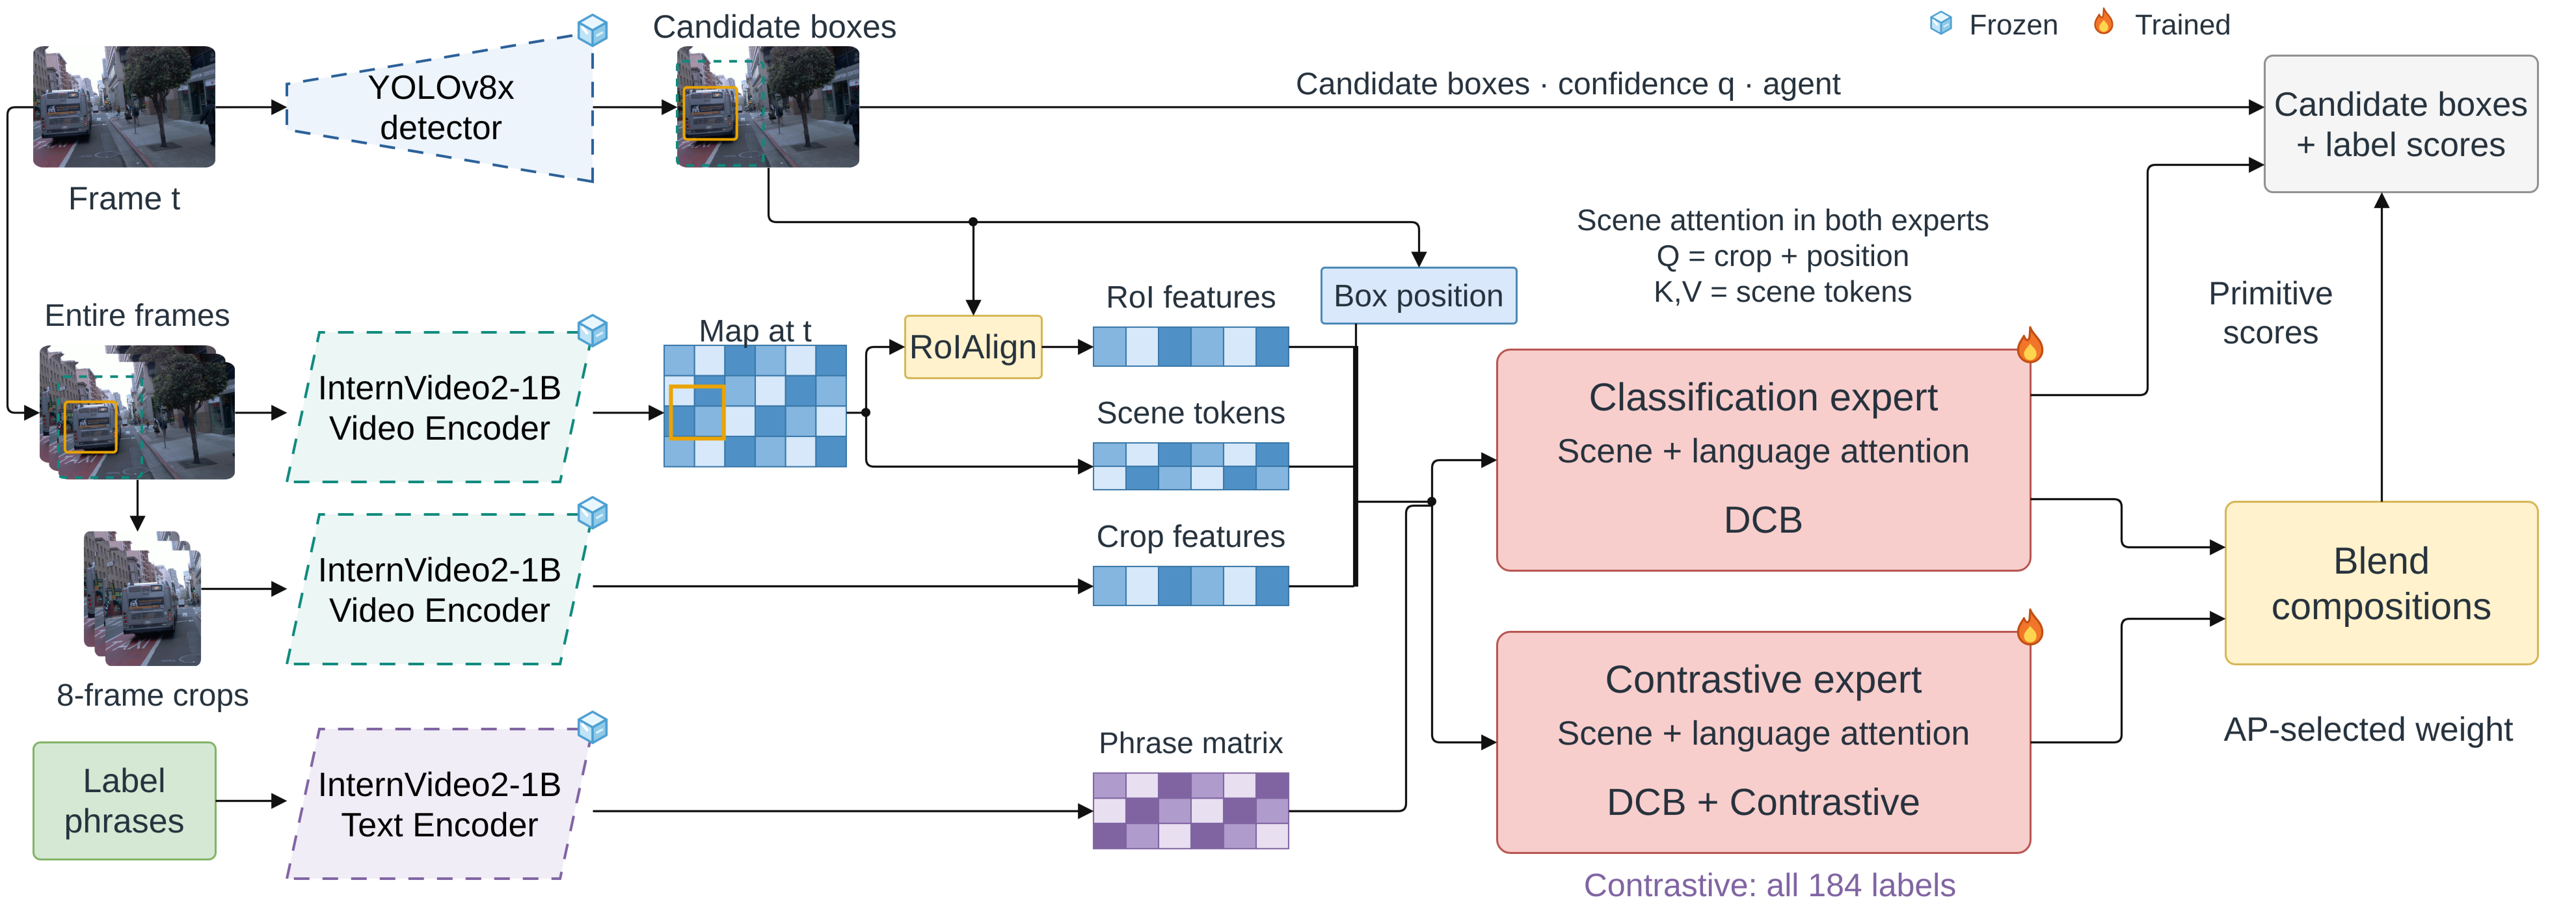
\includegraphics[width=\textwidth]{scaled-expert-blend.png}
\caption{CSEB with scaled frozen encoders. The classification expert uses DCB; the contrastive expert adds all-184 visual--phrase alignment. Both experts contain scene and language attention. YOLO supplies localization and agent outputs. The ROAD-Waymo imagery illustrates processing and is not a reported qualitative prediction \cite{road-waymo}.}
\label{fig:system}
\end{figure}

\subsection{Candidate and contextual representations}
Each candidate is associated with eight frames from $t-3$ to $t+4$, clamped at video boundaries. The crop is a fixed spatial window, with default width and height doubled around the candidate before clipping and resizing to $224\times224$. This is not a tracked tube. Frozen keyframe tokens supply a 1024-dimensional descriptor for the original visual encoder, or 1408 dimensions for the scaled encoder. The future frames make this contextual detection rather than causal anticipation.

A separate frozen entire-frame pass supplies actor-region RoIAlign features and 16 pooled scene tokens. Geometry consists of normalized corners, center, width, and height. Projections and a geometry MLP map these sources to width 512. With projected crop $c$, region $r$, scene tokens $S$, and geometry $g$, actor-conditioned scene attention and visual fusion are
\begin{align}
s&=\operatorname{MHA}(c+g,S,S),\\
v&=\operatorname{LN}\big(c+\operatorname{MLP}([c,r,s,g])\big).
\end{align}
The mean-pool control replaces scene attention by the average of the projected scene tokens. Both variants retain the crop residual. Attention uses eight heads; geometry enters the downstream head, not the frozen encoder.

\subsection{Language readout and auxiliary alignment}
The fixed ordered phrase bank contains 184 entries: agentness, 10 agents, 22 actions, 16 locations, 49 duplexes, and 86 triplets. A trainable residual text adapter produces adapted phrase vectors $T$. The original phrase width is 512; the scaled paired text model supplies 768-dimensional vectors projected to the head width. A gated language residual produces the joint feature,
\begin{equation}
j=\operatorname{LN}\big(v+\sigma(\beta)\operatorname{MHA}(v,T,T)\big).
\end{equation}
Normalized visual--phrase similarities $u_k=\cos(v,T_k)$ provide a second language-derived input. A $1208\rightarrow512\rightarrow184$ MLP predicts logits from $[j,c,u]$. The explicit crop bypass remains in this classifier.

For positive-label set $Y_i$ and rows $I_+$ with at least one positive label, the corrected all-184 auxiliary is
\begin{equation}
\mathcal L_{\mathrm{con}}=-\frac{1}{|I_+|}\sum_{i\in I_+}\frac{1}{|Y_i|}\sum_{k\in Y_i}
\log\frac{\exp(\cos(v_i,T_k)/0.07)}{\sum_{m=1}^{184}\exp(\cos(v_i,T_m)/0.07)}.
\end{equation}
The contrastive expert uses $\mathcal L_{\mathrm{cls}}+0.001\mathcal L_{\mathrm{con}}$. All-zero background rows remain in classification but are excluded from the auxiliary. Gradients reach the visual and text adapters while the pretrained encoders remain frozen. Both experts use language at inference; classification-only denotes the absence of the auxiliary loss, not the absence of language.

\subsection{Dynamic balancing and probability blending}
The focal baseline uses class-dependent alpha weighting and focusing parameter two. DCB replaces this objective with weighted binary cross-entropy. For sigmoid probability $p_{ik}$ and binary target $y_{ik}$,
\begin{equation}
B_{ik}=0.5+y_{ik}(1-p_{ik})+h_k,\qquad
\mathcal L_{\mathrm{DCB}}=\frac{1}{184N}\sum_{i,k}B_{ik}\operatorname{BCE}(\ell_{ik},y_{ik}).
\end{equation}
The detached history $h_k$ is the mean positive residual accumulated over previous batches, zero before any positive example is observed. History persists across epochs. This implementation averages over box--class entries; DCB replaces rather than multiplies the focal and alpha terms.

For composition label $k$, CSEB uses
\begin{equation}
p_{\mathrm{blend},k}=(1-w)p_{\mathrm{cls},k}+wp_{\mathrm{con},k}.
\end{equation}
A single weight per seed is selected from $\{0,0.125,\ldots,1\}$ using triplet crop AP on 45 reserved training videos, with ties favoring smaller $w$. It remains fixed at inference. Action and location scores remain with the classification expert; emitted agentness and agent identity come from YOLO. Event probabilities are multiplied by detector confidence once after blending. For illustration, $p_{\mathrm{cls}}=.20$, $p_{\mathrm{con}}=.80$, and $w=.75$ yield $.65$; confidence $.90$ yields an emitted score $.585$. These numbers illustrate arithmetic, not measured model predictions or calibrated event probabilities.

\section{Experimental Protocol}
ROAD-Waymo provides 600 training and 198 validation videos in the annotated partitions used here. The evaluation restricts comparison to 36,717 frames shared by the candidate and feature sources. Frame-level AP uses class-specific matching at IoU 0.5 and an interpolated precision envelope \cite{voc}. We report detector mAP, not the crop AP used for checkpoint selection. YOLO candidate generation uses confidence 0.001, NMS IoU 0.7, and at most 300 candidates per frame.

Tail membership is fixed from training counts. For $l_k=\log_{10}n_k$, define $z_k=(l_k-\mu)/\sigma$ over the 86 triplets. The 47 classes with $z<0$ form the tail, the nested 28 with $z<-0.5$ form the deeper tail, and the remaining 39 are common. These definitions characterize training frequency, not driving risk.

Crop heads use ten epochs of Adam with learning rate $.001$ and batch size 16,384. Video-grouped two-fold out-of-fold predictions train composition heads; full-data heads supply evaluation inputs. Contextual studies use 420 expert-training, 90 development, and 90 reserved gate videos. Expert training uses three epochs, batch size 256, learning rate $10^{-4}$, and weight decay $.01$. Development triplet crop AP selects the checkpoint; the same 45-video half of the gate partition selects blending. Seeds 0, 1, and 2 are repeated for the crop and contextual studies. Historical Stages 0--3 are single runs. Crop-to-context comparisons also change schedule and partition and therefore compare complete systems.

The scaled system uses the released InternVideo2-CLIP-1B paired checkpoints. Both visual and text encoders change, with an added $768\rightarrow512$ text projection. Cache computation also changes from the original FP16 path to BF16 encoder computation with float32 preprocessing/pooling and float16 feature storage. Thus, the scaling comparison cannot isolate visual parameter count. No independent annotated test evaluation is reported.

\section{Results}
\subsection{Crop composition and language controls}
The historical controlled Stage 2-to-3 change raises triplet mAP from 6.65\% to 9.73\%, keeping boxes and primitive outputs fixed. With original InternVideo2 features, the phrase classifier achieves 9.07\% triplet and 5.77\% tail mAP. Stage 5 reaches 11.23\% and 6.16\%; adding phrase-composition scores in Stage 6 reaches 11.28\% and 6.17\%, with deeper-tail mAP decreasing from 4.77\% to 4.57\%. The additional phrase path does not supply a large standalone improvement.

The original contextual head provides a more direct language test. Table~\ref{tab:language-controls} compares real phrases against explicit downstream language bypass and fixed random prototypes. Real phrases improve the tail mean by 0.43 points over bypass and 0.53 over random prototypes. Overall gains are small. Bypass changes active capacity, and random prototypes differ in geometry as well as semantic content. Three seeds and these interventions do not isolate linguistic meaning or establish equivalence when a contrast is unresolved.
\begin{table}[htbp]
\centering
\caption{Original-encoder language controls: mean $\pm$ sample SD (\%), three seeds.}
\label{tab:language-controls}
\begin{singlespace}
\begin{tabularx}{\textwidth}{@{}Xrrr@{}}
\toprule
\textbf{Condition} & \textbf{Triplet} & \textbf{Tail 47} & \textbf{Deep 28} \\
\midrule
Real phrases & $12.02\pm0.42$ & $6.19\pm0.59$ & $4.48\pm1.15$ \\
Language bypass & $11.88\pm0.28$ & $5.76\pm0.62$ & $4.27\pm0.89$ \\
Random prototypes & $11.88\pm0.42$ & $5.65\pm0.63$ & $4.02\pm0.72$ \\
\bottomrule
\end{tabularx}
\end{singlespace}
\end{table}

\subsection{Context, contrastive supervision, and loss}
Table~\ref{tab:context-original} reports original-encoder contextual variants. Mean pooling reaches 11.74\% triplet mAP, but its tail result is below crop Stage 6. Actor-guided attention improves the within-family comparison to 12.02\% triplet and 6.19\% tail. Adding the auxiliary increases overall mAP by .10 points while reducing tail by .40. The focal blend reaches 12.58\% triplet and 6.49\% tail, supporting complementarity rather than a uniformly stronger contrastive expert.
\begin{table}[htbp]
\centering
\caption{Original-encoder contextual triplet mAP (\%), three-seed means.}
\label{tab:context-original}
\begin{singlespace}
\begin{tabularx}{\textwidth}{@{}Xrrrr@{}}
\toprule
\textbf{Condition} & \textbf{All 86} & \textbf{Tail 47} & \textbf{Deep 28} & \textbf{Common} \\
\midrule
Mean pool, focal & 11.74 & 5.47 & 3.58 & 19.29 \\
Attention, focal & 12.02 & 6.19 & 4.48 & 19.06 \\
Attention, focal + contrastive & 12.12 & 5.79 & 3.85 & 19.75 \\
Attention blend, focal & 12.58 & 6.49 & 4.74 & 19.93 \\
Attention, DCB & 12.90 & 5.84 & 4.08 & 21.40 \\
Attention, DCB + contrastive & 12.88 & 5.81 & 4.20 & 21.40 \\
Attention blend, DCB & 13.43 & 6.23 & 4.54 & 22.10 \\
\bottomrule
\end{tabularx}
\end{singlespace}
\end{table}

Replacing focal with DCB raises the original-encoder blend to 13.43\% triplet mAP, but reduces tail and deeper-tail means relative to the focal blend. Dynamic weighting therefore does not automatically solve rare-class recognition. The negative frequency-group outcomes are retained rather than treating the development sequence as monotonic improvement.

\subsection{Scaled expert blending}
Tables~\ref{tab:scaled-all} and~\ref{tab:scaled-tail} report the final system. CSEB reaches 15.75\% triplet, 9.00\% tail, and 6.35\% deeper-tail mAP. It improves each triplet group over either constituent expert within every matched seed. The mean gains over classification alone are .72, .60, and .30 points, respectively. This is stronger evidence for expert complementarity than the modest standalone contrastive difference.
\begin{table}[htbp]
\centering
\caption{Scaled contextual detector f-mAP (\%), three-seed means.}
\label{tab:scaled-all}
\begin{singlespace}
\begin{tabular}{@{}lrrr@{}}
\toprule
\textbf{Output} & \textbf{Classification} & \textbf{Contrastive} & \textbf{CSEB} \\
\midrule
Agentness & 65.36 & 65.36 & 65.36 \\
Agent & 35.25 & 35.25 & 35.25 \\
Action & 24.75 & 24.85 & 24.75 \\
Location & 29.64 & 29.88 & 29.64 \\
Duplex & 23.37 & 23.53 & 24.36 \\
Triplet & 15.03 & 15.08 & 15.75 \\
\bottomrule
\end{tabular}
\end{singlespace}
\end{table}

\begin{table}[htbp]
\centering
\caption{Scaled contextual triplet groups: mean $\pm$ sample SD (\%).}
\label{tab:scaled-tail}
\begin{singlespace}
\begin{tabularx}{\textwidth}{@{}Xrrr@{}}
\toprule
\textbf{Condition} & \textbf{Triplet} & \textbf{Tail 47} & \textbf{Deep 28} \\
\midrule
Classification & $15.03\pm0.21$ & $8.40\pm0.58$ & $6.05\pm0.54$ \\
Contrastive & $15.08\pm0.30$ & $8.53\pm0.63$ & $5.99\pm0.53$ \\
CSEB & $15.75\pm0.27$ & $9.00\pm0.64$ & $6.35\pm0.57$ \\
\bottomrule
\end{tabularx}
\end{singlespace}
\end{table}

Relative to the original-encoder DCB blend, scaling improves overall triplet mAP by 2.32023 points using unrounded means. The disjoint-group identity
\begin{equation}
\Delta\mathrm{mAP}_{86}=\frac{47}{86}\Delta\mathrm{mAP}_{47}+\frac{39}{86}\Delta\mathrm{mAP}_{39}
\end{equation}
assigns 1.51155 points to the tail and .80868 to common classes. Approximately 65\% of the overall gain thus comes arithmetically from the tail. This is not a causal attribution to a particular module, and the nested deeper-tail group is not added a second time.

\subsection{Qualitative ranking evidence}
Figure~\ref{fig:case} illustrates a measured original-crop-study seed-0 case. A large-vehicle candidate at a junction has IoU .679, yet the first successful-match ranks are 288, 81,918, and 4,708 for Stages 4, 5, and 6. A descriptive top-615 class budget retains the phrase-classifier match but not the composition-head matches. Stage 6 improves this instance relative to Stage 5 while failing to preserve Stage 4's ranking. This is a ranking diagnostic, not evidence that localization failed.
\begin{figure}[htbp]
\centering
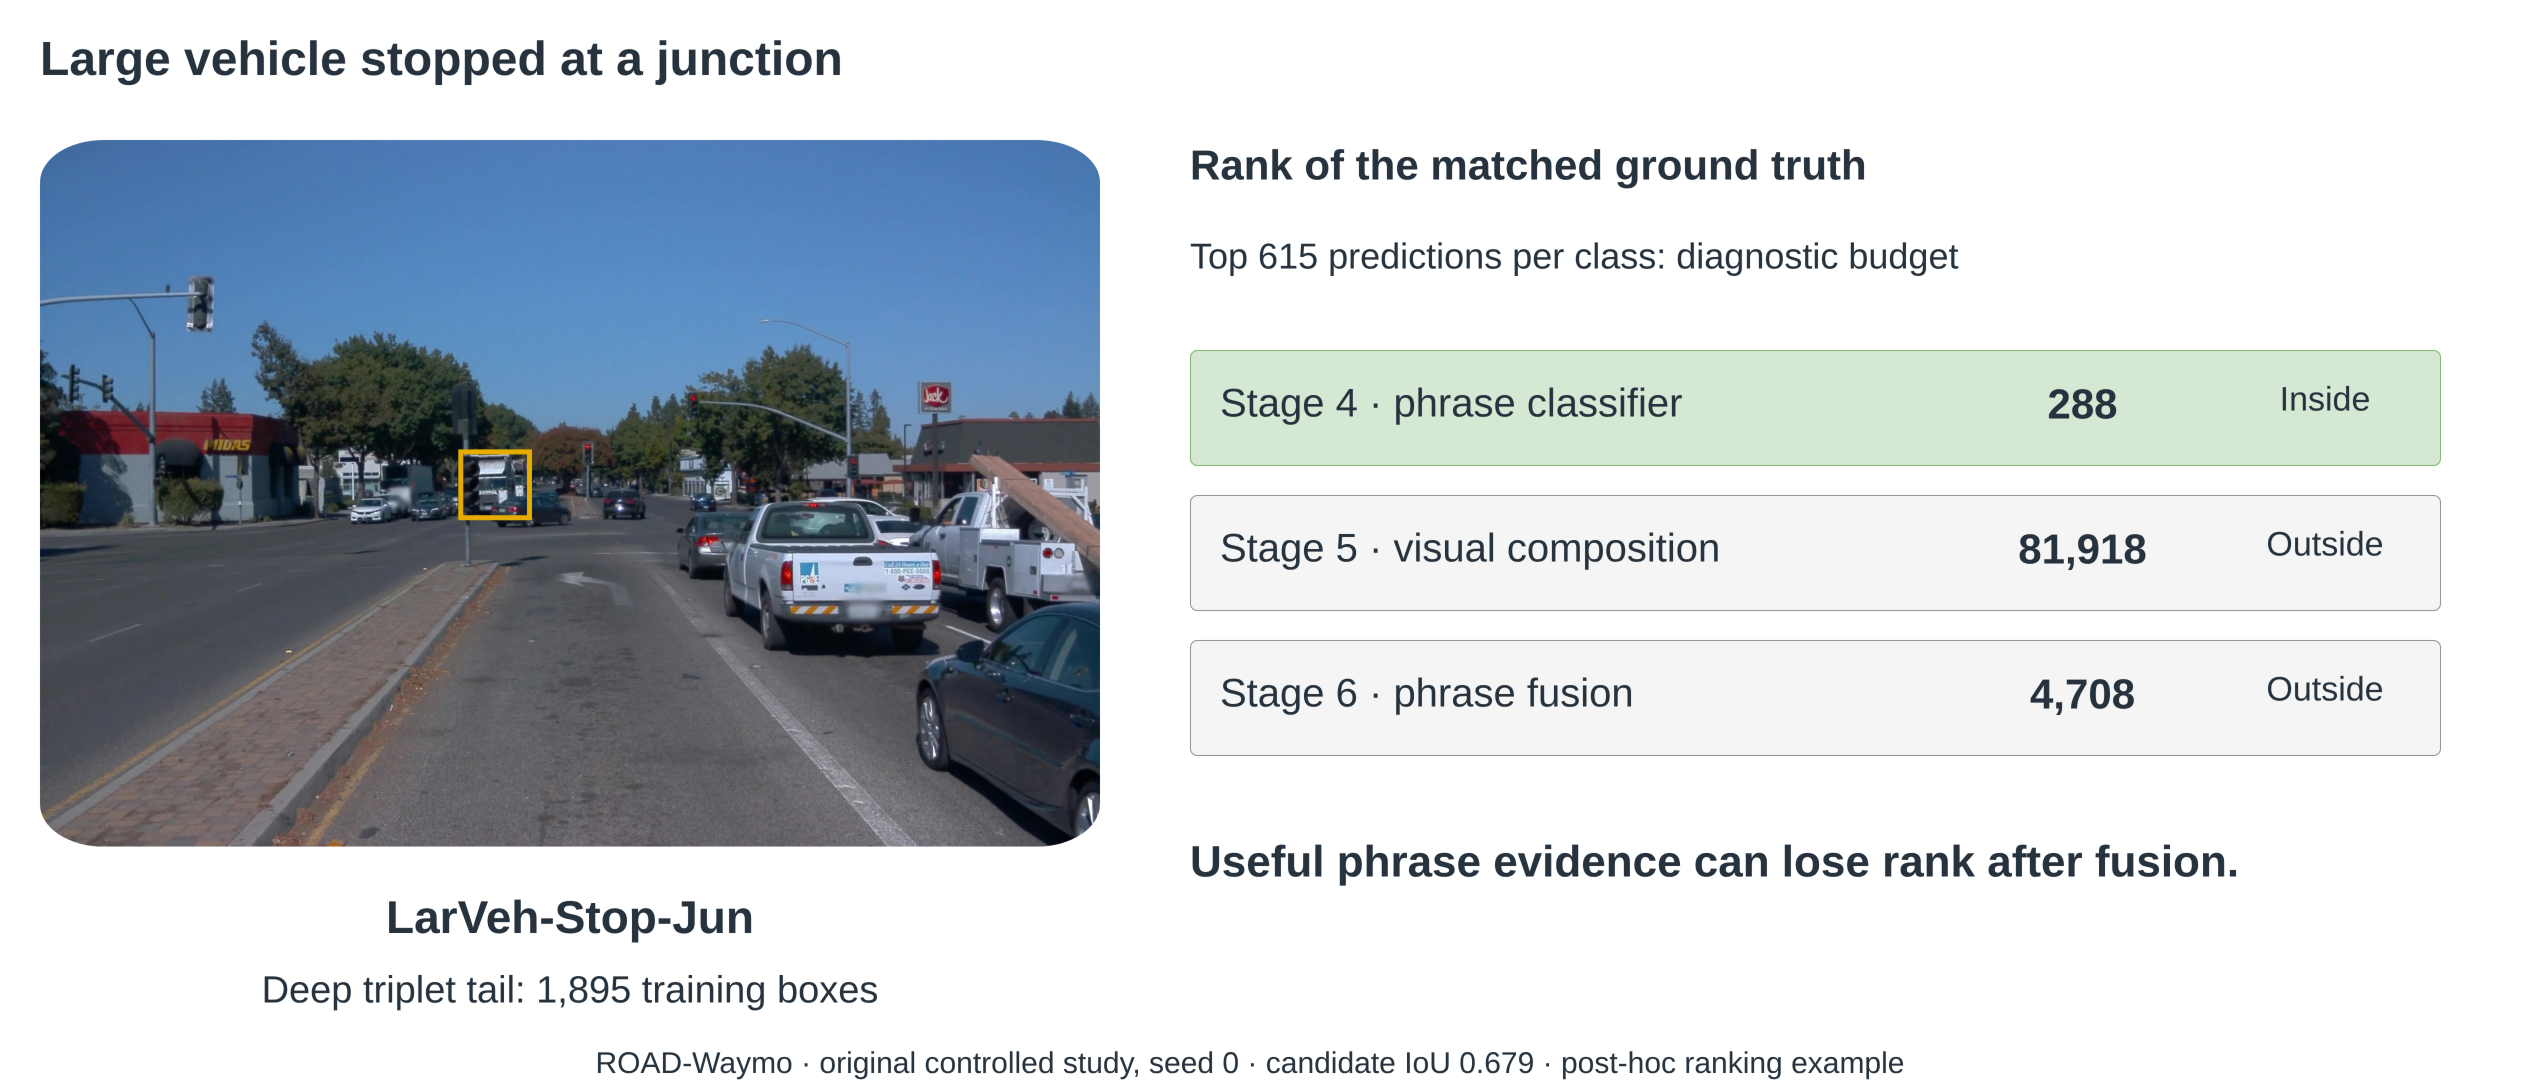
\includegraphics[width=\textwidth]{qualitative-tail-ranking.png}
\caption{Post-hoc ROAD-Waymo example from the original-encoder crop study, seed 0. The class has 1,895 training boxes. The diagnostic budget equals its evaluation ground-truth count, not a deployment threshold. No claim is made that contextual CSEB rescues this case.}
\label{fig:case}
\end{figure}
A second case, Bus-Stop-VehLane, has successful-match ranks 101, 2,878, and 325 under a top-583 budget. Stage 6 restores an included match relative to Stage 5 but still ranks it later than Stage 4. These deliberately selected contrasting examples explain heterogeneous effects; they do not estimate prevalence or replace full-population AP.

\subsection{Logical consistency versus recognition accuracy}
Valid composition labels do not guarantee agreement with independent primitive outputs. As an explicitly synthetic example for one candidate, let Bus-Stop-VehLane, Bus, Stop, and VehLane scores be 0.80, 0.90, 0.15, and 0.85. An illustrative 0.5 threshold selects the triplet but omits Stop, violating the implication from a triplet to all of its constituents. This is a teaching example, not a measured prediction or the AP decision rule. A selected Car agent paired with a Bus triplet likewise gives a conflicting description. Conversely, a consistently predicted stopped bus can still be wrong against car ground truth. ROAD-Waymo's multi-label locations also mean that junction and incoming-lane labels can legitimately coexist. The recorded ranking examples do not quantify these conflicts. A full-vector audit with a declared decision rule is needed before claiming a violation rate or improvement in logical consistency; CSEB is not a hard constraint system.

\subsection{Published reference results}
Table~\ref{tab:published} provides external reference values. The benchmark 3D-RetinaNet row comes from ROAD-Waymo; other external best-result rows are reported by FRCB \cite{road-waymo,frcb}. CSEB is a three-seed mean. Candidate generation, filtering, training, and frame selection differ, and comparable published tail results are unavailable. These values therefore contextualize the task rather than establish matched superiority.
\begin{table}[htbp]
\centering
\caption{Published references and CSEB detector f-mAP (\%); protocols differ.}
\label{tab:published}
\begin{singlespace}
\begin{tabularx}{\textwidth}{@{}Xrrrrr@{}}
\toprule
\textbf{Model} & \textbf{Agent} & \textbf{Action} & \textbf{Loc.} & \textbf{Duplex} & \textbf{Triplet} \\
\midrule
3D-RetinaNet (benchmark) & 15.57 & 12.30 & 12.40 & 10.50 & 6.20 \\
SlowFast & 17.45 & 15.35 & 14.42 & 9.66 & 5.51 \\
MViT & 20.75 & 13.10 & 15.41 & 10.17 & 6.63 \\
MViTv2 & 25.72 & 15.31 & 19.26 & 10.92 & 7.06 \\
MeMViT & 29.27 & 18.84 & 26.11 & 12.09 & 7.28 \\
STMixer & 24.70 & 17.12 & 20.98 & 15.16 & 9.33 \\
CycleACR (SlowFast) & 33.86 & 25.23 & 32.80 & 17.17 & 10.06 \\
FRCB & 33.64 & 23.87 & 32.33 & 17.84 & 11.71 \\
CSEB (ours, mean) & 35.25 & 24.75 & 29.64 & 24.36 & 15.75 \\
\bottomrule
\end{tabularx}
\end{singlespace}
\end{table}

\section{Discussion and Limitations}
The experiments distinguish three questions: whether candidates are localized, whether useful semantic evidence is available, and whether the trained readout preserves that evidence in the rankings used by AP. Better boxes alone do not answer the latter questions. Phrase supervision can help a constrained classifier while contributing only small or adverse changes after fusion. Complementary experts offer a way to retain useful differences, but their benefit must be assessed against the individual experts under matched seeds and data.

The final system is limited by development reuse of validation results. Although checkpoints and blend weights use reserved training partitions, validation findings informed subsequent research choices. Three seeds quantify optimization variability on a fixed population, not generalization to new environments. Original-encoder phrase controls do not establish the same mechanism in the scaled system. Paired-encoder and precision changes confound a capacity-only interpretation.

The fixed vocabulary does not test unseen compositions, and independent outputs do not guarantee logical consistency. The eight-frame window includes future context. End-to-end latency, memory usage, causal operation, and driving decisions are not evaluated. A prototype video can demonstrate execution and output interpretation but cannot substitute for those measurements. Follow-up work should isolate the scaled language branch, evaluate independent data, and quantify the complete inference path before deployment claims.

\section{Conclusion}
CSEB combines candidate-centered visual evidence, scene context, phrase representations, and separately trained contextual experts for ROAD-Waymo event detection. The final three-seed means reach 15.75\% triplet and 9.00\% tail mAP under the stated shared-frame protocol. The development sequence also reveals nonmonotonic rare-class effects: additional phrase scores, contrastive training, and DCB do not uniformly improve the tail. The most consistent final comparison supports expert complementarity. These results motivate further controlled evaluation of semantic and contextual integration rather than attributing the gains to a single component.
\printbibliography
\end{document}
